\documentclass[10pt]{article}

\usepackage[letterpaper,margin=1in]{geometry}
\usepackage[T1]{fontenc}
\usepackage[utf8]{inputenc}
\usepackage{newtxtext}
\usepackage{microtype}
\usepackage{graphicx}
\usepackage{booktabs}
\usepackage{tabularx}
\usepackage{array}
\usepackage{enumitem}
\usepackage{xcolor}
\usepackage{amsmath}
\usepackage{newtxmath}
\usepackage[font=small,labelfont=bf]{caption}
\usepackage{float}
\usepackage{tikz}
\usetikzlibrary{arrows.meta,positioning,fit,calc}
\usepackage{pgfplots}
\usepackage{pgfplotstable}
\pgfplotsset{compat=1.18}
\usepackage{url}
\usepackage[hidelinks]{hyperref}
\usepackage{cite}

\hypersetup{
  pdftitle={Who Authorized This Commit? PAPER and the Case for Governance-Native AI Communication},
  pdfauthor={Patrick Rho},
  pdfsubject={An open, product-integrated protocol for governance-native AI communication},
  pdfkeywords={AI governance, provenance, coding agents, open protocol, capability security, vLLM, SGLang}
}

\linespread{1.04}
\setlist{leftmargin=*,topsep=4pt,itemsep=2pt,parsep=1pt,partopsep=1pt}
\setlength{\parindent}{0pt}
\setlength{\parskip}{5pt plus 1pt minus 1pt}
\setlength{\textfloatsep}{18pt plus 3pt minus 3pt}
\setlength{\floatsep}{14pt plus 2pt minus 2pt}
\renewcommand{\arraystretch}{1.18}
\definecolor{paperink}{HTML}{263746}
\definecolor{paperblue}{HTML}{DCE8F0}
\definecolor{paperblueedge}{HTML}{58758A}
\definecolor{paperamber}{HTML}{E2A23A}
\definecolor{paperamberlight}{HTML}{FFF1D6}
\definecolor{papergray}{HTML}{EEF1F3}
\newcolumntype{Y}{>{\raggedright\arraybackslash}X}
\newcommand{\papername}{PAPER}
\newcommand{\system}{PCCP}

\title{\textbf{Who Authorized This Commit?}\\\large PAPER and the Case for Governance-Native AI Communication}
\author{Patrick Rho\\Patty Co., Ltd.}
\date{August 2026}

\begin{document}
\maketitle

\begin{abstract}
An AI coding agent can read a private repository, choose what leaves the machine, select a model, request tools, rewrite a file, and produce a commit. Yet after the commit exists, a basic accountability question remains difficult to answer: \emph{who was authorized to cause it?} Today's systems can usually recover pieces of the answer from API credentials, gateway decisions, tool logs, and Git history. They cannot reliably show that the same bounded authority governed the entire path from human intent to model invocation to executable side effect. This limitation motivates an authority-bearing exchange rather than independently correlated records.

We present \papername{} (Patty AI Provenance \& Enforcement Relay), a stateful protocol that makes governance part of AI communication itself. Its core primitive, the \emph{Governed Exchange}, binds an enrolled peer and human identity to a short-lived Capability Lease, an immutable Policy Epoch, inline Relay Verdicts, a server-authoritative model package and endpoint, and a content-addressed Provenance Spine. The result is a live exchange in which a model may propose an action but cannot manufacture the authority to execute it, and in which evidence is produced along the causal path rather than reconstructed afterward.

PAPER is provided as an open specification and an implemented system spanning the protocol core, Relay, Control Plane, PIA, policy, model registry, leases, and provenance. The official Patty Code Harness uses PAPER for service inference, while reusable PIA interfaces support vLLM, SGLang, and custom engines. A common semantic layer represents chat, streaming, tools, structured output, multimodal input, caching, and compaction, enabling the same protocol to serve coding agents and other AI applications. On an Apple M4 Pro, a comparison bundle comprising a 1~KiB record round trip, evidence-chain update, object digest, and Ed25519 sign-and-verify totals 43.45~$\mu$s. This equals 0.0097\% of MLPerf Inference's 450~ms interactive LLM time-to-first-token criterion, a difference of more than four orders of magnitude~\cite{mlperf2025llm}. At 1~MiB, record encode/decode reaches 10.81~GB/s. These results show that governance state and cryptographic evidence can be incorporated into the communication protocol with a small measured primitive cost relative to an interactive inference latency budget.
\end{abstract}

\section{Introduction}

Consider a plausible incident. A developer asks an agent to repair a failing authorization test. The agent selects six repository files as context, invokes a model advertised as ``Model A,'' receives a shell-tool proposal, runs a migration, edits two files, and creates a commit. Hours later, the migration is found to have exposed tenant data. The organization now asks:

\begin{itemize}
  \item Which human and which installed agent initiated the work?
  \item Was that agent allowed to disclose those six files to that model?
  \item Which immutable policy version permitted the migration command?
  \item Did the model merely propose the command, or did an authorized runtime execute it?
  \item Which exact model package and serving endpoint produced the proposal?
  \item Which parts of the final commit survived from model output after human edits?
\end{itemize}

Each component may maintain a log, but those records describe different boundaries. API authentication identifies a caller; a gateway records routing or policy decisions; a sandbox records execution; and Git records the resulting artifact. Reconstructing a single causal and authorization account therefore requires correlating records produced under different identifiers, time sources, retention policies, and trust assumptions. Gaps or ambiguities may become visible only after the side effect has occurred.

This fragmentation reflects a \emph{protocol-model gap}. Conventional AI interfaces transport prompts, tokens, tool calls, tasks, and artifacts without representing the bounded authority under which those objects may cause effects. Governance consequently remains external middleware rather than a condition on protocol state transitions. PAPER incorporates identity, authority, policy, and causal evidence into the inference and action lifecycle.

\papername{} addresses this gap through an authority-bearing exchange. A protected exchange advances only when the relevant identity, purpose, lease, policy epoch, model resolution, and Relay decision agree; the existence of a TLS connection or model-generated tool call is insufficient. Figure~\ref{fig:overview} summarizes this protocol structure.

\begin{figure*}[t]
  \centering
  
\includegraphics[width=0.96\textwidth]{figures/qwen-governed-exchange.png}
  \caption{Comparison of retrospective governance and PAPER's governed exchange. PAPER represents bounded authority, enforcement, model identity, and causal evidence as conditions of the live path. The illustration is conceptual and contains no empirical data.}
  \label{fig:overview}
\end{figure*}

\subsection{Contributions}

The paper examines the thesis that \emph{an agentic AI protocol should carry messages and actions together with the authority and causal evidence that make those actions legitimate}. It makes four contributions:

\begin{enumerate}
  \item \textbf{Governed Exchange.} We define a protocol lifecycle in which human and peer identity, purpose-bound Capability Lease, immutable Policy Epoch, model authority, and inline Relay Verdict are prerequisites for protected actions. A model proposal is data; execution authority remains external to the model.
  \item \textbf{Causal authority chain.} We connect user-facing model choice to a signed model package and leased endpoint, and connect intent, disclosure, inference, tool activity, edits, and artifacts through a content-addressed Provenance Spine and signed receipt. This construction provides a verifiable account of the authority under which an effect occurred.
  \item \textbf{Product-integrated reference system.} We implement the complete product path across the official Patty Code Harness, PAPER Relay, Control Plane services, PIA, serving-engine adapters, runtime authority, and provenance. The official Harness registers PAPER as its service-inference provider and sends Catalog Model identity rather than arbitrary provider URLs or inference API keys.
  \item \textbf{Open integration surface.} We publish an openly implementable specification, protocol library, PIA SDK, reusable vLLM and SGLang adapters, and a custom-engine boundary. Chat applications, copilots, automation systems, and other AI products can adopt the same governed exchange without inheriting Patty Code's application logic.
\end{enumerate}

The contribution is compositional. Secure transport, capabilities, provenance DAGs, signed receipts, and tool protocols already exist; PAPER integrates their authority semantics into one live state machine at the Harness--Relay--inference/runtime boundary. This integration makes governance enforceable before an effect and produces evidence as a protocol output.

\section{The Governance Gap in Agentic AI Communication}

The motivating incident exposes three mismatches that recur in agentic systems.

\paragraph{Authentication is not authorization history.}
A valid API credential can establish who opened a request without establishing which repository, purpose, tool class, model artifact, or side effect that identity was authorized to use throughout a long-running task. Agentic work outlives individual requests and crosses components whose authorization models are rarely identical.

\paragraph{Model output is not execution authority.}
Tool-calling formats make a proposed action machine-readable. They do not make it legitimate. If a model can cause execution merely by emitting the right syntax, untrusted repository text can attempt to acquire authority through prompt injection. The enforcement boundary must distinguish \emph{proposal}, \emph{approval}, and \emph{execution} as different events with different principals.

\paragraph{Logs record events; they do not necessarily prove one causal path.}
Correlated identifiers help, but correlation is not the same as a protocol-enforced chain. A durable answer to ``who authorized this commit?'' must bind the action to the authority and policy that existed \emph{before} execution, then preserve how its result changed through later human and automated work.

These mismatches suggest a missing layer between secure transport and application-specific governance: an exchange abstraction that carries identity, bounded authority, immutable policy, enforcement decisions, and evidence as coordinated protocol state.

\section{Adjacent Systems and Novelty Boundary}

\paragraph{Model APIs and gateways.}
HTTPS/JSON and streaming model APIs are effective request/response interfaces. Gateways can add authentication, quotas, policy, and logging. \papername{} differs primarily in the unit of state: authorization and evidence are bound to a long-lived governed session and exchange rather than reconstructed from independent middleware events.

\paragraph{MCP and A2A.}
The Model Context Protocol (MCP) standardizes interactions between AI applications and context/tool providers~\cite{mcp2025}. Agent2Agent (A2A) standardizes agent discovery, tasks, messages, and artifacts~\cite{a2a2026}. MCP can operate behind a governed tool broker, and A2A can operate at an agent-to-agent boundary. \papername{} targets the distinct boundary between a human-facing engineering Harness, inline policy enforcement, controlled inference/runtime infrastructure, and software provenance.

\paragraph{Runtime governance and agent security.}
MI9 examines integrated runtime governance for agentic systems~\cite{wang2025mi9}; AgentDojo provides an environment for prompt-injection attacks and defenses~\cite{debenedetti2024agentdojo}; and argument-level provenance work highlights the mismatch between coarse authorization and tool arguments~\cite{fan2026granularity}. \papername{} is complementary: it defines protocol objects and state transitions through which identity, policy, tool authority, and evidence can be enforced and exported.

\paragraph{Supply-chain provenance.}
in-toto records signed metadata about supply-chain steps~\cite{torresarias2019intoto,intoto}, while SLSA defines provenance expectations for build and source tracks~\cite{slsa12}. SCITT defines transparency services for registering signed statements about digital artifacts and issuing receipts~\cite{rfc9943}. \papername{} addresses an earlier interactive phase, before a build artifact necessarily exists: it governs whether context, inference, and side effects may occur. A \papername{} receipt may later become an in-toto/SLSA attestation input or a SCITT statement, but artifact transparency does not replace live exchange authority.

\paragraph{Identity and cryptographic building blocks.}
SPIFFE provides workload-identity conventions~\cite{spiffe}. \papername{} reuses TLS~1.3~\cite{rfc9846}, QUIC~\cite{rfc9000}, deterministic CBOR~\cite{rfc8949}, COSE~\cite{rfc9052}, HPKE~\cite{rfc9180}, and COSE receipts~\cite{rfc9942}. These standards provide transport and object-security primitives; they do not define the application-level authority model proposed here.

The novelty boundary follows from these roles: MCP describes tools, A2A describes inter-agent tasks, SPIFFE identifies workloads, gateways enforce policy, and in-toto attests supply-chain steps. PAPER binds these adjacent concerns through a governed state machine at the transition from proposed computation to an authorized, durable effect.

\section{Requirements and Threat Model}

\subsection{Design requirements}

The incident questions become six protocol requirements: (R1) bind every protected action to an enrolled peer and human identity; (R2) constrain authority with short-lived, purpose-bound grants; (R3) bind every enforcement decision to an immutable policy revision; (R4) identify the served model artifact and endpoint more strongly than a caller-supplied name; (R5) separate model proposal from runtime authorization and execution; and (R6) emit causal evidence that survives beyond ordinary application logs.

The system must also operate with a temporarily unavailable control plane. Relays therefore consume signed or authenticated snapshots, revocation state, policy epochs, model catalogs, and leases. Availability under stale state is bounded by explicit expiration and deployment policy rather than implicit cache behavior.

\subsection{Adversaries and non-goals}

We consider network attackers, unregistered clients, stolen or replayed credentials, compromised Harnesses, prompt-injected content, malicious tool output, model-name spoofing, cross-tenant mistakes, and evidence tampering. A Relay or administrator may also be malicious or compromised. The protocol aims to make such authority and evidence boundaries explicit; it cannot make a trusted plaintext Relay unable to inspect content, prove that a model behaved correctly, or prevent a fully compromised endpoint from acting outside the protocol. Hardware attestation and formal verification are optional assurance profiles, not assumptions required by the core protocol.

\section{The Governed Exchange}

The Governed Exchange is PAPER's unit of accountable AI work. It is larger than an API request and smaller than an entire developer session. It begins when a Harness declares a protected purpose and ends with a receipt that commits to the resulting evidence. Within that boundary, inference, context disclosure, model selection, tool use, approval, and output are transitions of one authority-aware state machine.

A useful mental model is a transaction whose commit condition is governance rather than database consistency. TLS answers whether bytes arrived through a protected channel. The Governed Exchange additionally asks whether the sender, purpose, policy, model, and proposed effect agree. Failure at a required gate prevents the protected transition; it is not merely recorded for later review.

\subsection{Architecture and peers}

The administrative Control Plane enrolls identities, issues policy and model state, manages revocation, and indexes evidence. It is authoritative but is not placed synchronously on every token. A Relay terminates Harness connections, validates cached signed state, performs inline policy decisions, routes approved inference, and appends evidence. A Patty Inference Agent (PIA) is a registered peer in front of a serving engine. The PIA translates PAPER's semantic request into a local engine interface; a raw model endpoint is never routing authority for the Harness. A runtime executes tools only after an independent authorization transition.

\begin{table*}[t]
\centering
\caption{Core authority and identity objects. Objects visible to the Harness are intentionally separated from deployment identities.}
\label{tab:objects}
\small
\begin{tabularx}{\textwidth}{@{}l l Y Y@{}}
\toprule
Object & Authority & Purpose & Important distinction \\
\midrule
Peer credential & enrollment authority & Binds key, peer profile, tenant, and validity & Identifies software instance, not merely user \\
Capability Lease & policy authority & Grants bounded action/model/tool/context scope & Permission; not resource capacity \\
Policy Epoch & policy authority & Immutable effective policy revision & Exchange binds to a digest, not ``latest'' \\
Catalog Model & model catalog & Stable user-facing service identity & Contains no provider endpoint \\
Model Descriptor & model catalog & Declares semantic capabilities and client minimums & Negotiation, not authorization by itself \\
Model Package (PMP) & model authority & Signed artifact/template/quantization identity & Stronger than human-readable model name \\
Endpoint Lease & serving authority & Binds active PIA endpoint to approved package & Short-lived deployment state \\
Account Capacity Lease & capacity authority & Coordinates distributed workload slots & Capacity; distinct from action permission \\
\bottomrule
\end{tabularx}
\end{table*}

\subsection{Protocol enforcement and retrospective logging}

A log schema can describe an allow decision but cannot require that the decision precede disclosure, model allocation, or tool execution. PAPER represents identity binding, lease presentation, epoch binding, verdict, dispatch, tool authorization, and closure as ordered protocol transitions. Peers must complete these transitions before protected work advances, distinguishing protocol enforcement from retrospective middleware records.

More precisely, let $a$ be a protected action attempted during exchange $x$ at time $t$. PAPER permits the corresponding state transition only when

\begin{equation}
\operatorname{advance}(x,a,t) = P_x \land S_x \land L_x(a,t)
  \land E_x \land V_x(a) \land R_x(a),
\label{eq:advance}
\end{equation}

where $P_x$ and $S_x$ denote valid peer and session bindings, $L_x(a,t)$ is an unexpired Capability Lease covering $a$, $E_x$ is a recognized immutable Policy Epoch, and $V_x(a)$ is an allowing Relay verdict. $R_x(a)$ collects action-specific authority: inference requires an approved model package and live endpoint lease, while a side effect requires independent tool authorization. Equation~\ref{eq:advance} is a protocol acceptance condition, not a formal security proof; failure of any conjunct blocks the protected transition.

\subsection{Transport and representation}

QUIC is the preferred binding because independent streams reduce head-of-line coupling; TLS~1.3 over TCP is the fallback. Both use the same application semantics and ALPN identity. Records contain a fixed prelude, canonical header, payload, logical lane identifier, and lane sequence. Deterministic CBOR provides reproducible object encoding. COSE signatures protect credentials, leases, epochs, model manifests, and receipts where object-level verification is required.

Application authentication binds the peer credential, nonces, negotiated profile, and channel context so that a credential proof captured on one connection cannot be replayed on another. PAPER defines these messages, and the product path performs the handshake. Section~\ref{sec:implementation} distinguishes the local-development credential profile from the organization-issued, revocation-aware, transcript-bound verification profile used for stronger deployment assurance.

\section{Authorization State Transitions}

\subsection{Identity, sessions, and Capability Leases}

User identity, Harness identity, and workload/session identity are separate because they answer different questions: who requested the work, which software installation carried it, and which bounded activity is now in progress. Enrollment gives a Harness a peer credential; it does not grant inference or tool authority. A Working Session binds user, Harness, organization/project, purpose, repository, and effective policy. A Capability Lease then grants a subset of actions for a short interval: permitted models, context paths, tool classes, token budget, and approval requirements. Revocation or expiration prevents new protected actions even if the underlying transport remains healthy.

\subsection{Policy Epoch and Relay Verdict}

A Policy Epoch freezes the meaning of ``allowed'' for an exchange. It is an immutable, digest-addressed snapshot rather than a pointer to whatever policy happens to be current when an auditor asks. If policy changes mid-session, active work follows an explicit continue, rebind, pause, or terminate rule; its historical meaning does not silently change. Before protected content reaches a PIA or runtime, the Relay emits a structured verdict such as allow, deny, transform, quarantine, or require approval. The verdict identifies the epoch and rule set that produced it.

\subsection{Exchange lifecycle}

A typical exchange progresses through \textsc{open}, \textsc{governance}, \textsc{route}, \textsc{stream}, optional \textsc{tool/approval}, and \textsc{close}. These states are not descriptive labels; they constrain which messages are legal. The Relay validates the peer/session binding, Capability Lease, Policy Epoch, catalog model, model package, endpoint lease, and capacity state before dispatch. Token or data records are multiplexed over lanes with sequence numbers. Side-effecting actions carry an idempotency class so reconnect/resumption cannot silently duplicate a completed operation.

Applied to the motivating incident, the context disclosure is allowed or denied under the lease and epoch before six files leave the Harness. ``Model A'' resolves to a signed package and leased PIA endpoint before inference. The shell string remains a proposal until a separately authorized runtime transition executes it. The final receipt binds these decisions to the evidence root later associated with the commit.

Figure~\ref{fig:lifecycle} makes the ordering explicit. The optional branch is whether a tool is proposed; authorization of a proposed tool is never optional.

\begin{figure}[H]
  \centering
  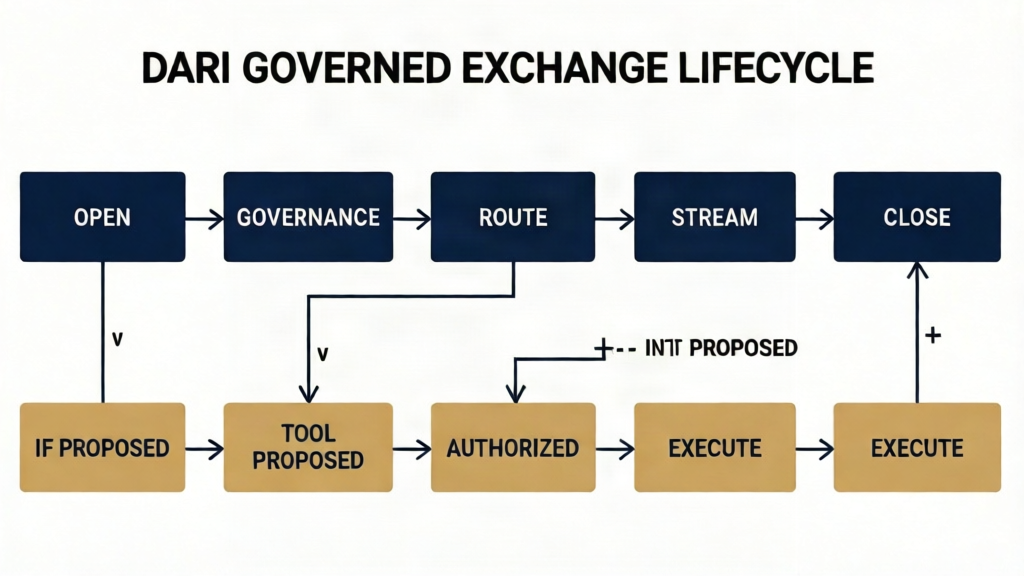
\includegraphics[width=\textwidth]{figures/governed-exchange-lifecycle.png}
  \caption{Protocol-design view of a Governed Exchange. Protected work advances through ordered authority gates; a model-generated tool proposal enters an optional branch but requires an independent authorization transition before execution. This figure specifies intended semantics, not measured implementation coverage.}
  \label{fig:lifecycle}
\end{figure}

\subsection{Server-authoritative model resolution}

PAPER treats user-facing model names and security identities as distinct, and separates:

\begin{equation*}
\text{Catalog Model} \rightarrow \text{PMP} \rightarrow \text{PIA Endpoint}.
\end{equation*}

After authentication, the Harness receives an effective model catalog scoped by entitlement, organization policy, deployment profile, geography, and client capability. A Model Descriptor advertises semantic features---for example multimodal input, structured output, parallel tools, caching, reasoning controls, and resumability---without exposing an endpoint. An inference-open message references the Catalog Model and Catalog Epoch. The Relay rejects stale or unauthorized selections, resolves a signed Patty Model Package (PMP), and selects a PIA endpoint with a valid lease. These are three deliberately different identities: the Catalog Model is the stable product visible to the user, the PMP identifies the approved artifact and serving configuration, and the Endpoint Lease identifies where that package may run now. A caller may express a preference; it cannot turn a string or base URL into trusted infrastructure.

Figure~\ref{fig:model-identity} shows how that separation prevents a user-visible name from becoming routing authority.

\begin{figure}[H]
  \centering
  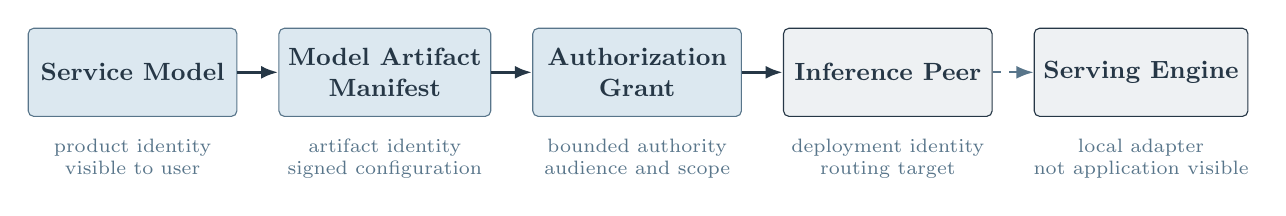
\begin{tikzpicture}[
  font=\small,
  identity/.style={draw=paperblueedge, fill=paperblue, rounded corners=2pt,
    minimum width=2.65cm, minimum height=1.12cm, align=center,
    text=paperink, font=\small\bfseries},
  runtime/.style={draw=paperink, fill=papergray, rounded corners=2pt,
    minimum width=2.65cm, minimum height=1.12cm, align=center,
    text=paperink, font=\small\bfseries},
  resolve/.style={-{Latex[length=2.2mm]}, very thick, draw=paperink},
  local/.style={-{Latex[length=2.2mm]}, thick, dashed, draw=paperblueedge},
  kind/.style={font=\scriptsize, text=paperblueedge, align=center}
]
  \node[identity] (catalog) {Service Model};
  \node[identity, right=0.52cm of catalog] (manifest) {Model Artifact\\Manifest};
  \node[identity, right=0.52cm of manifest] (grant) {Authorization\\Grant};
  \node[runtime, right=0.52cm of grant] (peer) {Inference Peer};
  \node[runtime, right=0.52cm of peer] (engine) {Serving Engine};

  \node[kind, below=0.16cm of catalog] {product identity\\visible to user};
  \node[kind, below=0.16cm of manifest] {artifact identity\\signed configuration};
  \node[kind, below=0.16cm of grant] {bounded authority\\audience and scope};
  \node[kind, below=0.16cm of peer] {deployment identity\\routing target};
  \node[kind, below=0.16cm of engine] {local adapter\\not application visible};

  \draw[resolve] (catalog) -- (manifest);
  \draw[resolve] (manifest) -- (grant);
  \draw[resolve] (grant) -- (peer);
  \draw[local] (peer) -- (engine);
\end{tikzpicture}

  \caption{Protocol-design view of server-authoritative model resolution. Product, artifact, and deployment identities remain distinct until the Relay resolves them to an enrolled PIA; the serving engine is a local implementation detail, not a Harness-selectable endpoint.}
  \label{fig:model-identity}
\end{figure}

\subsection{Tool authority and prompt injection}

PAPER applies the following rule to prompt-injected output: \emph{model output is a proposal, never authority}. Tool descriptors specify execution placement, risk class, argument schema, approval policy, idempotency, and provenance requirements. Incrementally streamed arguments are not executable until complete and authorized. Repository text, chat, files, and tool output retain trust labels but cannot enlarge lease scope. Injected text must therefore cross an independently controlled authority boundary. PAPER records both the proposal and the decision that allowed, transformed, or denied execution.

\section{Causal Provenance and Receipts}

The audit objective is to establish how an artifact arose under a particular authority. The Provenance Spine represents causal edges among human intent, selected context, policy decisions, model invocation, output, tool proposal, approval, execution result, edits, tests, review, and source-control artifacts. Nodes are content-addressed and typed; edges describe causation, derivation, disclosure, transformation, or binding. The absence of a required transition leaves a verifiable gap in the causal account. Events performed entirely outside the governed path remain outside the receipt's observation boundary.

For compact exchange integrity, let $r_0=H(\textsf{domain}\parallel\textsf{exchange-open})$ and

\begin{equation}
r_i = H(\textsf{domain}\parallel r_{i-1}\parallel H(e_i)),
\end{equation}

where $e_i$ is the canonical representation of evidence event $i$. A signed Evidence Receipt binds the final root to the exchange, identities, policy epoch, model/package resolution, outcome, and retention/export profile. The receipt is deliberately compact: an auditor given the complete ordered event sequence can recompute the root and verify consistency with the closed exchange. Proving an arbitrary selectively disclosed subset requires an additional commitment or inclusion-proof construction; the current chain primitive alone does not provide it.

The construction provides tamper evidence under explicit component trust assumptions. A compromised authorized component can emit false source data, and a coalition controlling every signer can manufacture a consistent account. Cross-component receipts and external transparency reduce unilateral trust but cannot establish the factual accuracy of source events. Cryptographic integrity and semantic truth are therefore treated as separate properties.

Selective-export profiles may replace sensitive nodes with commitments or redacted summaries, but their verifiable linkage is a design requirement rather than a property established by the current chain benchmark. Source-code attribution after refactoring or merging is probabilistic and should carry confidence and transformation history rather than a binary ``AI-generated'' label.

\section{From Open Specification to Integrated Product}
\label{sec:implementation}

PAPER is published as an open specification and implemented as the communication substrate of the PCCP product system. The implementation includes a 32-byte record prelude, bounded headers and payloads, deterministic CBOR, COSE Sign1, Ed25519 object signatures, content-addressed digests, evidence chains, peer/session state machines, TLS/TCP and QUIC bindings, model/catalog schemas, policy and lease services, Relay and PIA services, provenance, registries, conformance surfaces, and deployment manifests. The benchmark snapshot is repository commit \texttt{0234034}; the product integration described below reflects the subsequent Patty Code and PCCP integration.

\subsection{Integration with Patty Code}

The official Patty Code Harness registers PAPER as its service-inference provider. It opens a PAPER connection, negotiates the Harness profile, receives the Relay challenge, sends the protocol authentication proof, and carries inference through \texttt{AI\_OPEN}, streaming token records, and \texttt{AI\_COMPLETE}. Official builds register no generic OpenAI-, Anthropic-, or Responses-style provider for Patty service inference. The Harness selects a server-issued Catalog Model; arbitrary base URLs and raw inference API keys do not constitute routing authority. These constraints are enforced by the current provider registration and protocol client.

The Relay evaluates the governed request and forwards authorized inference to a PIA over the PAPER boundary. PIA translates the normalized semantic request to the local serving engine and returns normalized text, reasoning, tool-call, usage, and completion events. The Harness runtime also supplies repository access, approval modes, sandboxed tools, session recovery, MCP tools, skills, subagents, and editor integration. PAPER is therefore exercised within the operational lifecycle of the integrated coding-agent product.

\subsection{Application-neutral integration}

The protocol is application-neutral at the semantic boundary. Its AI layer represents multi-turn messages, streaming, tool definitions and calls, structured output, multimodal input, cache controls, and compaction. A chat application can use the message-and-stream subset; a copilot can add context and tool capabilities; an automation system can bind durable effects and evidence. None must import Patty Code's repository or user-interface logic.

The open integration surface includes the protocol library, a PIA SDK and examples, reusable vLLM and SGLang adapters, and an \texttt{EngineAdapter} boundary for custom runtimes. PIA preserves a stable trust boundary while allowing serving engines to evolve independently: \texttt{Relay <-> PAPER <-> PIA <-> local engine}. This avoids requiring a permanent vLLM or SGLang fork and makes the protocol usable by commercial and open-source AI applications alike.

\begin{table*}[t]
\centering
\caption{Implemented product surface and the evidence used in this paper. Product availability and empirical measurement scope are reported separately.}
\label{tab:claims}
\small
\begin{tabularx}{\textwidth}{@{}Y l Y Y@{}}
\toprule
Product surface & Availability & Integration evidence & Scope of claim \\
\midrule
Open PAPER core & Available & specification, protocol library, registries, transport and object tests & Implemented protocol and reusable library \\
Official Patty Code Harness & Integrated & PAPER-only provider registration and Harness protocol client & Patty Code uses PAPER for service inference \\
Relay and Control Plane & Integrated & identity, catalog, policy, lease, routing, audit, and provenance services & Product governance path exists; assurance depends on deployment profile \\
PIA and serving engines & Available & PAPER PIA plus reusable vLLM and SGLang adapters & Governed engines can be integrated without Harness endpoint authority \\
SDK and custom applications & Available & PIA SDK, examples, and custom \texttt{EngineAdapter} interface & Chat, copilots, automation, and custom AI products can adopt the protocol \\
Evidence and provenance & Integrated & ChangeSet, span, chain, receipt, and audit services & Causal evidence is a product output under stated trust assumptions \\
Measured core operations & Measured & five-run medians from the checked-in benchmark dataset & Primitive latency, throughput, allocation, and interactive-budget comparison \\
Assurance profiles & Profile-specific & conformance audit and explicit assurance matrix & Deployment requirements and validation depth are explicit \\
\bottomrule
\end{tabularx}
\end{table*}

\section{Evaluation Questions and Baselines}

The evaluation considers whether governance can be enforced while preserving interactive performance. It asks: (Q1) what connection and pre-inference latency does PAPER add; (Q2) how does Relay cost scale with streams; (Q3) what evidence and storage cost is associated with a verifiable causal path; (Q4) which adversarial cases are rejected by protocol state; and (Q5) how accurately provenance survives software evolution?

\subsection{Baselines}

We define five goal-aware baselines: B0, a minimal secure binary stream; B1, bearer-authenticated HTTPS/JSON streaming; B2, HTTPS/JSON plus comparable gateway policy and logging; B3, PAPER with identity/session and minimal governance; and B4, PAPER with lease, policy, content checks, verdicts, and provenance. The primary comparisons are B2 versus B4 (comparable governance, different lifecycle) and B3 versus B4 (the marginal cost of governance). MCP and A2A are treated as semantic neighbors rather than performance baselines.

End-to-end experiments must report connection p50/p95/p99, time to first Relay verdict, TTFT, inter-token latency, sustained throughput, CPU time, allocation, memory per stream, and evidence bytes. The environment disclosure must include CPU, memory, NIC, RTT, topology, OS, runtime and transport-library versions, model/quantization, GPU, policy modules, and storage backend.

\subsection{Security and provenance experiments}

Negative tests include an unknown peer, expired/replayed lease, unknown Policy Epoch, stale catalog, unapproved model package, invalid endpoint lease, profile-confused message, malformed state sequence, duplicate side effect after resume, prompt-injected capability escalation, and modified receipt. Provenance fidelity should be measured on generated functions followed by human edits, file renames, function moves, rebases, merges, and multi-agent changes. Precision/recall and confidence calibration are more appropriate than anecdotal examples.

\section{Measured System Primitives}

\subsection{Experimental setup}

This paper isolates PAPER's framing, cryptographic, and evidence operations so that their cost remains visible rather than being absorbed into network or model variance. Measurements ran locally on an Apple M4 Pro with 14 logical CPUs and 48~GiB RAM under macOS~27.0 on arm64. Each benchmark was repeated five times; Table~\ref{tab:microbench} reports the median. The resulting measurements provide a reproducible lower-layer baseline for the B0--B4 system comparisons.

For operation $o$, the reported latency is

\begin{equation}
\widetilde{t}_o = \operatorname{median}
  \left\{t_o^{(1)},t_o^{(2)},\ldots,t_o^{(5)}\right\}.
\label{eq:median}
\end{equation}

Only $\widetilde{t}_o$ was retained in the artifact. The five individual observations were not retained, so the paper does not report dispersion, confidence intervals, or statistical significance.

\begin{table}[t]
\centering
\caption{In-memory system-primitive medians over five runs. Record tests include encode and decode.}
\label{tab:microbench}
\small
\begin{tabular}{@{}l r r r@{}}
\toprule
Operation & Time/op & B/op & allocs \\
\midrule
Record, 1 KiB & 290.2 ns & 2,384 & 7 \\
Record, 64 KiB & 8.46 $\mu$s & 139,472 & 7 \\
Record, 1 MiB & 97.0 $\mu$s & 2,105,556 & 7 \\
CBOR Hello round trip & 599.4 ns & 592 & 9 \\
Evidence-chain update & 73.05 ns & 32 & 1 \\
1 KiB object digest & 403.1 ns & 32 & 1 \\
Ed25519 sign+verify & 42.7 $\mu$s & 64 & 1 \\
\bottomrule
\end{tabular}
\end{table}

Record encode/decode reaches 97.0~$\mu$s for a 1~MiB payload, while its time per byte falls across the three measured sizes as fixed work is amortized. For record payload size $s$, we define size-normalized cost and effective payload throughput as

\begin{align}
c(s) &= \frac{\widetilde{t}_{\mathrm{record}}(s)}{s},
  & q(s) &= \frac{s}{\widetilde{t}_{\mathrm{record}}(s)}.
\label{eq:normalized}
\end{align}

The measured $c(s)$ decreases from 0.283~ns/byte at 1~KiB to 0.0925~ns/byte at 1~MiB; equivalently, $q(s)$ rises from 3.53 to 10.81~GB/s (10.1~GiB/s). The 73.05~ns evidence-chain update is small enough to apply per evidence event, and a 42.7~$\mu$s sign-and-verify operation is practical at exchange or receipt boundaries.

To give these isolated numbers an application-level point of reference, we construct a comparison bundle from four primitives used across the governed-exchange lifecycle: 1~KiB record round trip, evidence-chain update, object digest, and Ed25519 sign-and-verify. Their arithmetic sum is

\begin{equation}
L_{\mathrm{PAPER},1\mathrm{KiB}}
= 0.2902 + 0.07305 + 0.4031 + 42.688
= 43.45435~\mu\mathrm{s}.
\label{eq:interactive-budget}
\end{equation}

MLPerf Inference uses a 450~ms 99th-percentile TTFT criterion for interactive Llama~2 70B serving~\cite{mlperf2025llm}. Relative to this reference,

\begin{equation}
\rho = \frac{L_{\mathrm{PAPER},1\mathrm{KiB}}}{450~\mathrm{ms}}
= 9.66 \times 10^{-5} = 0.0097\%.
\label{eq:budget-ratio}
\end{equation}

The reference budget is more than 10,000 times larger than the combined primitive cost. Ed25519 sign-and-verify accounts for 98.2\% of the bundle; PAPER's framing, digest, and evidence-chain operations contribute the remaining 0.77~$\mu$s. The measured core cost is therefore four orders of magnitude below the interactive LLM response budget used for comparison.

To expose memory cost separately, let $B_{\mathrm{op}}(s)$ be bytes allocated per record benchmark operation. Its allocation amplification is

\begin{equation}
A(s) = \frac{B_{\mathrm{op}}(s)}{s}.
\label{eq:allocation}
\end{equation}

$A(s)$ falls from 2.33 at 1~KiB to 2.01 at 1~MiB. The benchmark allocates an encoded buffer and decoded record on every iteration; the large-payload allocation is therefore approximately twice the payload size and identifies a concrete optimization target.

Figure~\ref{fig:primitive-latency} makes the four-order-of-magnitude range visible; Table~\ref{tab:microbench} remains the exact-value record.

\begin{figure}[H]
  \centering
  \pgfplotstableread[col sep=tab]{benchmark-data/core-primitives.tsv}\primitivebenchmarks
\begin{tikzpicture}
\begin{axis}[
  width=\textwidth,
  height=7.0cm,
  ybar,
  bar width=14pt,
  ymode=log,
  log basis y=10,
  ymin=50,
  ymax=200000,
  ylabel={Median latency (ns/op, log scale)},
  xtick=data,
  xticklabels={Record 1K,Record 64K,Record 1M,CBOR Hello,Evidence chain,1K digest,Ed25519},
  x tick label style={font=\scriptsize, rotate=35, anchor=east},
  y tick label style={font=\scriptsize},
  ylabel style={font=\small},
  grid=major,
  grid style={draw=papergray},
  axis line style={draw=paperink},
  tick style={draw=paperink},
  nodes near coords,
  nodes near coords style={font=\scriptsize, rotate=90, anchor=west, text=paperink},
  point meta=explicit symbolic,
  enlarge x limits=0.08,
]
\addplot+[fill=paperblueedge, draw=paperink]
  table[x expr=\coordindex, y=median_ns_per_op,
    meta=median_ns_per_op] {\primitivebenchmarks};
\end{axis}
\end{tikzpicture}

  \caption{Empirical median latency of the seven measured in-memory primitives, read directly from the checked-in TSV and shown on a logarithmic axis. The isolated view makes the protocol's CPU-side cost directly comparable with the interactive latency budget in Equation~\ref{eq:budget-ratio}.}
  \label{fig:primitive-latency}
\end{figure}

These primitives are the repeated building blocks for canonical evidence construction, indexing, retention, and signed receipts. Even before further allocation optimization, their combined 1~KiB cost consumes less than one ten-thousandth of the interactive TTFT reference budget, leaving substantial room for policy evaluation, transport, storage, and model serving.

The full repository suite passed at the evaluated commit. A separate coverage audit found that several conformance-test names exceed the properties exercised by their assertions. The package exposes tests named for invariants 1--5 and 7--12, with no named test for invariant 6; several passing tests exercise only a proxy for their stated property. For example, the Policy Epoch test checks connection readiness rather than unknown-epoch rejection, and the reconnect test contains no assertion. We therefore report repository test completion separately from invariant coverage. The detailed audit appears in Appendix~A.

\subsection{Interpretation}

The comparison bundle occupies 0.0097\% of the referenced interactive LLM latency target, while large-record processing exceeds 10~GiB/s. These measurements indicate that the evaluated primitive costs leave substantial latency budget for TLS/QUIC establishment, policy modules, database/cache access, content classifiers, network placement, model scheduling, and evidence storage. B0--B4 experiments can quantify those system-level components, while the negative-test suite evaluates whether the Relay converts PAPER's authority model into enforced denials.

\section{Comparative Scope}

\begin{table*}[t]
\centering
\caption{Scope-aligned qualitative comparison of PAPER and adjacent system families.}
\label{tab:comparison}
\small
\begin{tabularx}{\textwidth}{@{}l Y Y Y Y@{}}
\toprule
System family & Primary boundary & Live purpose-bound authority & Inline model/package identity & Interactive causal code provenance \\
\midrule
Model API & application--model service & typically application-defined & usually caller-visible model identifier & external \\
AI gateway & application--provider mediation & gateway/policy dependent & provider-route dependent & logs/plug-ins \\
MCP & AI application--tool/context provider & authorization is deployment-specific & not its objective & not its objective \\
A2A & agent--agent task/artifact exchange & protocol/task dependent & not its objective & not its objective \\
in-toto/SLSA & software supply-chain steps/artifacts & step/build policy & artifact identity & post-step/build provenance \\
\papername{} & Harness--Relay--PIA/runtime & Capability Lease + Policy Epoch & Catalog Model + PMP + Endpoint Lease & native exchange graph/receipt \\
\bottomrule
\end{tabularx}
\end{table*}

Table~\ref{tab:comparison} locates the contribution in composition and lifecycle semantics rather than lower-layer mechanisms. A conventional gateway could implement many PAPER concepts; the empirical distinction is whether deployment-specific middleware and shared protocol state produce different interoperability, authority-gap, and failure-behavior outcomes. The proposed B2--B4 comparison is designed to measure this distinction.

\section{Security Consequences of Externalizing Authority}

PAPER treats the model as an untrusted principal and constrains the authority available through its output channel. An unregistered generic client lacks a valid peer credential and session grant. A stolen Harness key remains bounded by lease lifetime, repository/purpose scope, revocation, and optional device evidence. A fake model name cannot select an endpoint when the Relay resolves only an authorized Catalog Model through a signed PMP and active Endpoint Lease. A prompt-injected tool call cannot grant itself authority because execution requires an independent lease/policy transition outside the model's output channel.

Replay protection requires transcript-bound authentication and idempotency evidence. Transport fallback must preserve the same authorization objects and state machine. Evidence tampering changes the chain root, while an attacker able to compromise all receipt signers can still forge a consistent account. A malicious inspectable Relay can read plaintext and may omit or distort events; cross-component receipts, limited retention, independent export, and optional payload protection reduce but do not eliminate this trust.

These security properties require the protocol's verification profile. The checked-in local-development profile uses self-signed certificates and simplified proof provisioning for installation convenience. The commercial profile specifies organization-issued peer credentials, certificate verification, revocation, and transcript-bound proof validation. The profiles share the integrated Harness--Relay--PIA product path but provide different assurance levels.

\section{Incremental Gateway Migration}

One protocol kernel supports public cloud, enterprise, and sovereign profiles by varying enabled modules, policy defaults, retention, mobility, and infrastructure placement rather than forking wire semantics. Sovereign deployments can use local PKI, catalogs, PIA endpoints, and offline-signed update bundles. Cross-vendor interoperability remains a distinct empirical claim and is not inferred from profile support.

PCCP supports brownfield adoption through caller inventory, additive catalog/control schemas, parallel observation beside a legacy gateway, dual recording of comparable requests, canary Harness cohorts, and rollback gates. Patty Code implements the migrated client boundary: the official Harness uses PAPER for service communication and exposes no generic model-provider fallback. Administrative APIs and PIA-local adapter APIs remain outside that Harness trust path by design.

\section{Discussion: Protocol Scope and Consequence Governance}

PAPER suggests that agent protocols should represent the consequences of messages in addition to their transport. Request authentication and application logs may be sufficient for systems that only return text. Systems that disclose private context, invoke tools, mutate repositories, and create durable artifacts also require authority over state transitions at the protocol boundary.

The protocol complements rather than absorbs adjacent standards. Its adoption criterion is the durability and privilege of an application's effects: a chat application can use identity, model authority, and evidence without enabling repository tools, while a coding agent can activate capabilities for durable state changes.

\paragraph{Application breadth.}
Inference, tools, context, files, chat, multimodal input, and directives share identity and session infrastructure while remaining capability-separated. This is what lets a conventional chat application adopt the same protocol core used by Patty Code without inheriting file mutation or tool execution authority.

\paragraph{State and operations.}
Leases, epochs, resumption, revocation, catalogs, and evidence add operational burden. Cache staleness and control-plane partitions require explicit fail-closed, bounded-stale, or degrade behavior. Binary framing also requires first-class diagnostics and capture tooling.

\paragraph{Privacy.}
Fine-grained provenance can become employee surveillance. Deployments need purpose limitation, minimization, role-separated access, retention bounds, selective export, and notice. Content-addressing does not anonymize sensitive content; unsalted hashes can enable guessing attacks.

\paragraph{Deployment and assurance profiles.}
The implemented product surface spans the complete Harness--Relay--PIA path, while its evidence is organized by assurance profile. The measured profile provides primitive latency, throughput, and allocation results; the commercial profile uses organization-issued peer credentials, certificate validation, revocation state, and transcript-bound proof verification; and the research matrix identifies the experiments that deepen scale, provenance-fidelity, interoperability, and formal-analysis evidence. This separation turns deployment obligations into explicit engineering choices instead of leaving them implicit in middleware configuration.

\paragraph{Formal analysis.}
The state machine and invariants are candidates for formal modeling. This paper provides no formal security proof; provenance establishes recorded causality under component assumptions rather than semantic correctness or authorship truth.

\section{Ethics and Surveillance Risk}

Evidence about prompts, files, tool use, edits, and human decisions can improve incident response and accountability while also enabling disproportionate monitoring. The protocol therefore supports retention and export profiles, but technical configurability is insufficient. Deployments should establish lawful purpose, employee notice, access review, appeal, data-subject handling, and a separation between security investigations and performance management. Public deployments should default to operationally minimal traces; regulated deployments should justify deeper retention per policy domain.

Generated conceptual artwork is used for Figures~\ref{fig:overview} and~\ref{fig:lifecycle}; both communicate protocol architecture and contain no measurement or factual comparison. Figure~\ref{fig:model-identity} is a LaTeX-native protocol-design diagram. Figure~\ref{fig:primitive-latency} and the empirical tables are derived from the checked-in benchmark dataset; the retained medians are reproducible from the benchmark harness, while new statistical claims would require publication of raw per-run output.

\section{Reproducibility}

The arXiv source package contains the exact LaTeX source, bibliography, conceptual figures, benchmark dataset, and build instructions. The open implementation repository contains the protocol library, Relay, PIA, Control Plane services, vLLM/SGLang adapters, PIA SDK examples, registries, benchmark harness, and deployment material; the Patty Code repository contains the official Harness integration. From the implementation repository root, the reported primitive measurements can be reproduced with:

\begin{quote}\small
\texttt{go test ./internal/paper -run '\^\$' -bench 'Benchmark(...)' -benchmem -count=5}
\end{quote}

where the artifact README provides the complete regular expression. The PDF builds offline with \texttt{latexmk} and BibTeX. Raw per-run output, network/load generators, topology automation, negative-security fixtures, provenance datasets, and independent implementation results are required only for the corresponding stronger statistical, scale, attack-resistance, fidelity, or interoperability claims.

\section{Conclusion}

Accountability for an AI-generated commit requires more than identifying the model that produced its tokens. It requires evidence that the path from human intent to durable effect remained within bounded authority across context disclosure, model resolution, tool authorization, and artifact creation.

PAPER represents this path as a Governed Exchange that binds identity, purpose, bounded capability, immutable policy, model and package resolution, inline enforcement, and causal evidence. Model output remains a proposal, while independent protocol transitions authorize protected effects. The resulting receipt records why those transitions were permitted and how their outputs reached an artifact.

The implementation comprises a protocol core and governance services, an official Patty Code Harness that uses PAPER for service inference, a Relay--PIA path, reusable vLLM and SGLang adapters, and an SDK boundary for chat, copilots, automation, and custom engines. The measured primitive bundle occupies 0.0097\% of the referenced interactive TTFT budget, and 1~MiB record processing reaches 10.81~GB/s. The assurance matrix reports the validation depth associated with each additional security and system-level claim.

Together, the specification, integrated implementation, and measured primitive costs support governance as a shared protocol property connecting applications, policy authorities, model infrastructure, tools, and causal evidence. This shifts authority over system effects from model output and deployment-specific convention to explicit, verifiable protocol state.

\bibliographystyle{abbrv}
\bibliography{references}

\clearpage
\onecolumn
\appendix
\section{Assurance Matrix for Research Invariants}

\noindent Table~\ref{tab:invariants} audits the conformance-test coverage at the evaluated commit. ``Weak'' denotes an assertion that does not exercise the full invariant stated by its test name; ``partial'' denotes a meaningful primitive or state check without a complete end-to-end path.

\begin{center}
\small
\refstepcounter{table}
\label{tab:invariants}
\textbf{Table \thetable: Coverage audit of the candidate research invariants.}\\[4pt]
\begin{tabularx}{\textwidth}{@{}c Y l Y@{}}
\toprule
ID & Candidate invariant & Coverage & Audit note \\
\midrule
I1 & No protected action before peer authentication & Partial & connection-state gating asserted; listener proof verification incomplete \\
I2 & No protected action outside a valid Capability Lease & Weak & test checks credential time validity, not action authorization \\
I3 & No action under an unknown Policy Epoch & Weak & test checks connection readiness, not epoch lookup/rejection \\
I4 & No invocation against an unapproved package/endpoint lease & Partial & signature mutation tested; full route binding not exercised \\
I5 & Tool proposal grants no authority by itself & Weak & test checks only a valid peer credential \\
I6 & Context disclosure requires explicit authority & Missing & no named conformance test \\
I7 & Transport fallback preserves authorization semantics & Weak & ALPN constant checked; fallback exchange not exercised \\
I8 & Reconnect does not duplicate completed side effects & Placeholder & named test has no assertion \\
I9 & Protected exchange terminates with verifiable evidence & Partial & deterministic chain checked; termination/receipt path not exercised \\
I10 & Provenance mutation changes digest & Implemented primitive & distinct content produces distinct domain-separated digest \\
I11 & Peer profiles cannot emit privileged messages & Placeholder & message list is constructed but not passed through enforcement \\
I12 & Administrative communication and enforcement are distinct & Structural & distinct message type codes asserted \\
\bottomrule
\end{tabularx}
\end{center}

\subsection{Evidence Required for Stronger Claims}

The following experiments extend the evidence associated with system-level performance, security, provenance, and interoperability claims:

\begin{enumerate}
  \item \textbf{Transport and authentication:} exercise full certificate and COSE proof verification, revocation, transcript binding, resumption, and QUIC-to-TCP fallback with p50/p95/p99 connection measurements.
  \item \textbf{End-to-end inference:} compare B0--B4 on identical payloads and model output, reporting Relay verdict latency, TTFT, streaming throughput, CPU, allocation, and memory.
  \item \textbf{Governance negatives:} reject expired/replayed leases, unknown epochs, stale catalogs, unapproved packages, invalid endpoints, profile-confused messages, and duplicate side effects through the actual Relay path.
  \item \textbf{Scale and failure:} measure concurrent sessions/streams, Relay restart, control-plane loss, bounded-stale caches, capacity-authority loss, and evidence-backend degradation.
  \item \textbf{Provenance fidelity:} publish a labeled dataset covering human edits, file/function moves, rebases, merges, and multi-agent changes with precision, recall, and confidence calibration.
  \item \textbf{Independent evidence:} demonstrate an implementation not sharing the same implementation stack, publish golden vectors/fuzz results, and obtain an external security review for the production-security profile.
\end{enumerate}

\end{document}
